\chapter{Arquitectura en capas}
Un sistema de comunicación se pueden diferenciar en distintos niveles en los que cada uno realiza una función independiente, pero que a su vez interactúan con los niveles limítrofes.

\begin{center}
    \vspace{-10pt}
    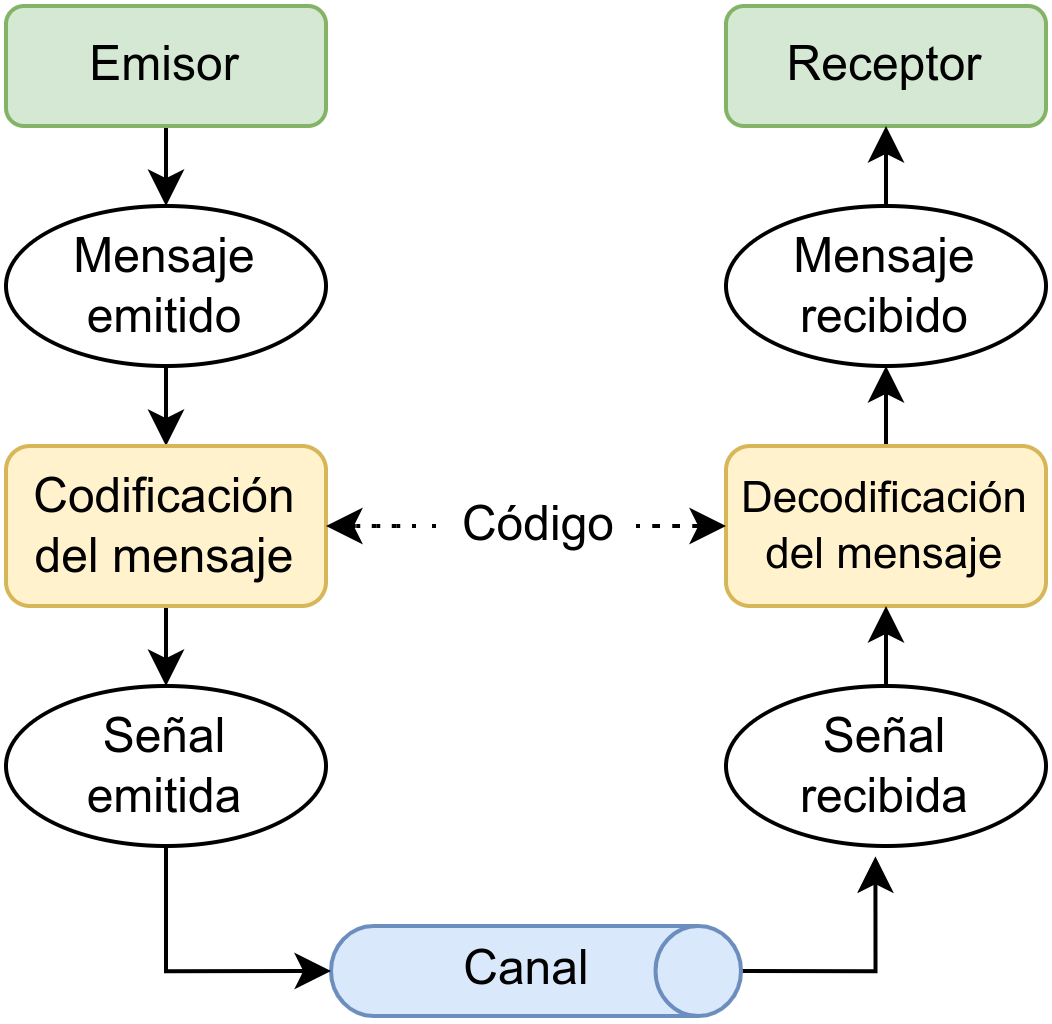
\includegraphics[width=0.4\linewidth]{comunicacion-esquema.png}
    \vspace{-10pt}
\end{center}

Este ejemplo es un modelo simplificado de comunicación, y dentro de una arquitectura de red de ordenadores pueden existir más capas en las que pueden existir distintas funciones extra que no aparecen en este esquema.

\section{Origen}

Al comienzo de las redes de ordenadores cada empresa creaba su propio sistema de comunicación creando su propio hardware y software, lo que hacía imposible la interconexión entre equipamiento de distintas empresas.

Estos sistemas de comunicación constan de unas reglas que los nodos deben conocer para poder comunicarse entre sí, y a ese conjunto de reglas se les denomina \textbf{protocolo de comunicación}.


Para que eso hoy en día no suceda ya que las redes están definidas en varios estándares, como veremos más adelante.

\infobox{Un \textbf{estándar} es un conjunto de normas que pueden abarcar distintos niveles (tanto software como hardware) que ha sido aceptado, o creado, por la gran mayoría de las empresas del sector para poder realizar la interconexión e intercomunicación entre sí.}


\section{Ventajas de la división en capas}

La división en capas nos permite:
\begin{itemize}
    \item Dividir el proceso de comunicación en procesos más pequeños.

    \item Aislar las funciones de cada capa. De esta manera, en caso de realizar modificaciones en la misma, no afecta al resto de capas.

    \item Ocultar la implementación al resto de capas. Siguiendo con el punto anterior, una capa utilizará los servicios de su capa inferior sin saber cómo realiza sus funciones.

    \item Cada capa puede constar de distintos estándares, facilitando la interconexión de distintas tecnologías
\end{itemize}

Una arquitectura de red en capas se implementa por medio de distintos protocolos, formando una familia de protocolos para facilitar la comunicación de distintos sistemas y equipos en la red.

\infobox{Una arquitectura en capas nos permite que cada capa actúe de manera independiente y que incluya sus propios protocolos. Cada capa dispone de una serie de servicios que ofrece a su capa limítrofe superior.}

Desde el comienzo de las redes de ordenadores han existido distintas familias de protocolos, y se puede considerar que hubo una \href{https://en.wikipedia.org/wiki/Protocol_Wars}{guerra de protocolos durante las décadas de 1970 a 1990}. Empresas, organizaciones y países se posicionaban sobre cuál sería el mejor protocolo de comunicaciones y el que saldría ganador para el uso a nivel internacional.

Por destacar algunos protocolos que ya no se usan:

\begin{itemize}
    \item \textbf{\href{https://en.wikipedia.org/wiki/Systems_Network_Architecture}{SNA}} creado en 1974 por IBM.
    \item \textbf{\href{https://en.wikipedia.org/wiki/NetBIOS_Frames}{NetBEUI}} de Microsoft. Que evolucionó a NetBIOS sobre TCP/IP que hoy día se usa en Windows Server.
    \item \textbf{\href{https://en.wikipedia.org/wiki/IPX/SPX}{IPX/SPX}} de Novell.
\end{itemize}

\section{Modelo de referencia OSI}
El modelo de interconexión de sistemas abiertos, conocido como “modelo \textbf{OSI}” (\textit{\textbf{O}pen \textbf{S}ystems \textbf{I}nterconnection} en inglés) es un \textbf{modelo de referencia (teórico)} que busca estandarizar las funciones de comunicación para un sistema informático siendo agnóstico a la tecnología utilizada para realizar la implementación y a los protocolos utilizados en cada capa.

El diseño comenzó en 1977 tratando de terminar con la \href{https://en.wikipedia.org/wiki/Protocol_Wars}{guerra de protocolos} comentada previamente, y la Organización Internacional de Estandarización (\textit{International Organization for Standardization}, o \textbf{ISO} en inglés)  terminó por definir el estándar ISO-7498 en 1984.


\subsection{Capas en el modelo OSI}
El modelo OSI está compuesto por siete capas numeradas del 1 al 7 siendo la 1 la más baja y haciendo referencia a la parte física de la red.


%TODO: modificar tabla?
\begin{yukitblr}{X X X[3,l]}
    Capa & Nombre de la unidad de datos & Función \\

    7ª - Aplicación & Datos
    & APIs de alto nivel, como compartir recursos y acceso remoto a archivos. \\

    6ª - Presentación & Datos
    & Traducción de datos entre un servicio de red y una aplicación, que incluye la codificación de caracteres, la compresión de datos y el cifrado y descifrado de datos.
    \\

    5ª - Sesión & Datos
    & Manejo de sesiones de comunicación, por ejemplo el continuo intercambio de información en forma de múltiples transmisiones hacia ambos lados entre dos nodos.
    \\

    4ª - Transporte & Segmento, Datagrama
    & Transmisión de segmentos de datos confiable entre puntos de red, incluyendo la segmentación, el acknowledgement y la multiplexación.
    \\

    3ª - Red & Paquete
    & Estructura y manejo de una red multinodo. Incluye el direccionamiento, el ruteo y el control de tráfico.
    \\

    2ª - Enlace de datos & Trama
    & Transmisión de datos confiable entre dos nodos conectados mediante una capa física.
    \\

    1ª - Física & Bit, Baudios
    & Transmisión y recepción de flujos de bits sin procesar por un medio físico.
    \\
\end{yukitblr}


\section{Pila de protocolos TCP/IP}

Durante el surgimiento de las redes de comunicaciones entre ordenadores cada fabricante creaba su propio estándar, lo que hacía que la comunicación entre ellos no fuese posible. En 1974  \href{https://en.wikipedia.org/wiki/Vint_Cerf}{Vint Cerf} and \href{https://en.wikipedia.org/wiki/Bob_Kahn}{Bob Kahn} describen un protocolo para compartir recursos usando envío de paquetes a través de una red de comunicación. Es el comienzo del protocolo \textbf{TCP}.

En 1984 fue el protocolo elegido por parte del Departamento de Defensa de Estados Unidos, y poco tiempo después se convirtió en el estándar de facto de la comunicación de red que posteriormente dio lugar a Internet.

Tal como se puede ver, la pila de protocolos TCP/IP es funcional, al contrario que ocurre con el modelo OSI que sólo es teórico.

La pila TCP/IP cuenta con cuatro capas:

\begin{yukitblr}{X X X[3,l]}
    Capa & Protocolos conocidos & Función \\

    4ª - Aplicación
    & HTTP, FTP, POP, SMTP, ...
    & Es la capa más cercana al usuario, utilizada por las aplicaciones a la hora de enviar datos
    \\

    3ª - Transporte
    & TCP, UDP
    & Estructura y manejo de una red multinodo. Incluye el direccionamiento, el ruteo y el control de tráfico.
    \\

    2ª - Red
    & IPv4, IPv6
    & Transmisión de datos confiable entre dos nodos conectados mediante una capa física.
    \\

    1ª - enlace
    & Ethernet, IEEE 802, 802.11 (wifi)
    & Es una mezcla de las capas 1 y 2 del modelo OSI.
    \\
\end{yukitblr}


\subsection{Protocolo TCP}

El objetivo del protocolo TCP es crear conexiones dentro de una red de datos compuesta por redes de ordenadores para intercambiar datos. La ventaja es que el protocolo busca garantizar que los datos son entregados a su destino sin errores y en el mismo orden en el que se transmitieron.

Por otro lado, también proporciona un mecanismo para distinguir distintas aplicaciones dentro de una misma máquina, a través del concepto de \textbf{puerto}.

Hoy día TCP es el protocolo más utilizado dentro de las aplicaciones que hacen uso de comunicación en red. Por ejemplo, los protocolos HTTP, SMTP, SSH, FTP... hacen uso de TCP como como protocolo de transporte (\textbf{capa 4 del modelo OSI}).


\subsubsection{Establecer comunicación}
A la hora de establecer una comunicación usando el protocolo TCP lo habitual es que en el lado del \textbf{servidor (el receptor de la comunicación)} exista un servicio que esté “\textit{escuchando}” en un puerto previamente levantado (por ejemplo, un servidor web que escucha en el \textbf{puerto 80 y 443}).

El cliente comenzará la comunicación enviando un paquete \textbf{SYN} a la IP del servidor y al puerto con el que se quiere comunicar, a lo que si todo ha ido bien, el servidor responderá con la respuesta \textbf{SYN/ACK}.
\begin{wrapfigure}{r}{0.35\linewidth}
    \hfill
    \vspace{-30pt}
    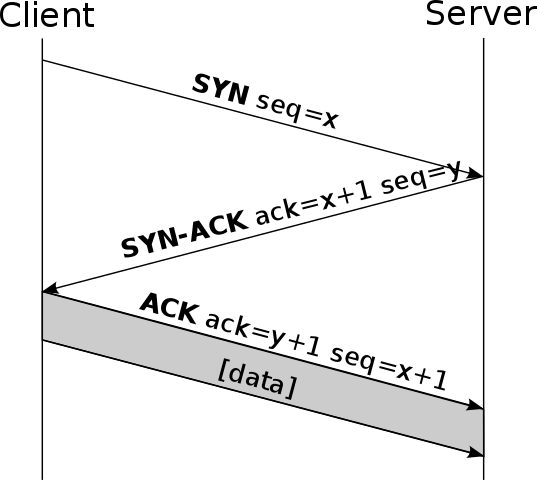
\includegraphics[width=0.9\linewidth]{tcp-handshake.png}
    \vspace{-10pt}
\end{wrapfigure}

Finalmente, el cliente debería responderle al servidor con un ACK, completando así la \textbf{negociación en tres pasos} (SYN, SYN/ACK y ACK) y la fase de establecimiento de conexión.

De esta manera, comenzará la transferencia de datos, a lo que se le añade una serie de mecanismos que determinan la fiabilidad y robustez del protocolo. Entre ellos están incluidos:


\begin{itemize}
    \item Uso del número de secuencia para ordenar los segmentos TCP recibidos y detectar paquetes duplicados.
    \item \textit{Checksums} para detectar errores.
    \item Indicación por parte del receptor que ha recibido los paquetes para detectar pérdidas.
    \item Temporizadores para detectar retrasos o necesidad de reenvío de información.
\end{itemize}


\subsubsection{Cierre de la comunicación}
\begin{wrapfigure}{r}{0.35\linewidth}
    \hfill
    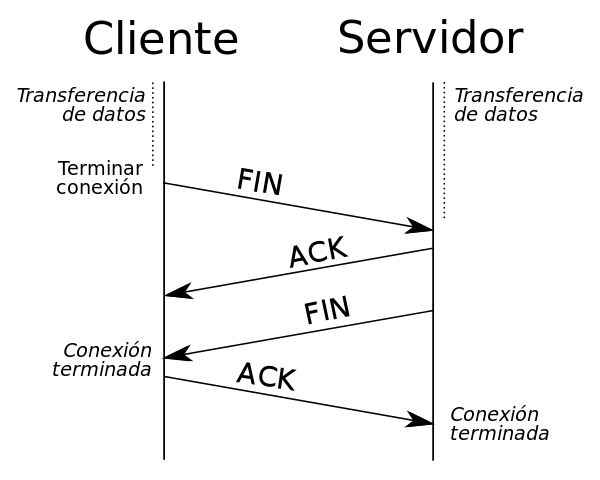
\includegraphics[width=0.9\linewidth]{tcp-fin.png}
    \vspace{-10pt}
\end{wrapfigure}
La fase de finalización de la conexión utiliza una negociación en cuatro pasos (four-way handshake), terminando la conexión desde cada lado independientemente.

Cuando uno de los dos extremos de la conexión desea parar su "mitad" de conexión transmite un segmento con el flag FIN en 1, que el otro interlocutor asentirá con un ACK. Por tanto, una desconexión típica requiere un par de segmentos FIN y ACK desde cada lado de la conexión.

Una conexión puede estar "medio abierta" en el caso de que uno de los lados la finalice pero el otro no. El lado que ha dado por finalizada la conexión no puede enviar más datos pero la otra parte si podrá.



\subsubsection{Puertos TCP}
TCP usa el concepto de número de puerto para identificar a las aplicaciones emisoras y receptoras. Cada lado de la conexión TCP tiene asociado un número de puerto (de 16 bits sin signo, con lo que existen 65536 puertos posibles) asignado por la aplicación emisora o receptora.

Los \textbf{puertos bien conocidos} son asignados por la Internet Assigned Numbers Authority (IANA), van del 0 al 1023 y son usados normalmente por el sistema o por procesos con privilegios. Algunos ejemplos son: FTP (21), SSH (22), Telnet (23), SMTP (25) y HTTP (80).

Los \textbf{puertos registrados} son normalmente empleados por las aplicaciones de usuario de forma temporal cuando conectan con los servidores, pero también pueden representar servicios que hayan sido registrados por un tercero (rango de puertos registrados: 1024 al 49151).

Los \textbf{puertos dinámicos/privados} también pueden ser usados por las aplicaciones de usuario, pero este caso es menos común. Los puertos dinámicos/privados no tienen significado fuera de la conexión TCP en la que fueron usados (rango de puertos dinámicos/privados: 49152 al 65535.